\subsection{Diagnostic: What is NOT Working}

\paragraph{Small-scale structure decorrelates, and this is fundamental.} SR
matches HR cell-by-cell at large scales ($r{=}0.95$ for $k<0.05$) but loses the
match at small scales ($r{=}0.40$ for $k>0.2$, Table~\ref{tab:srs-match}). This
is not a capacity bug: it is set by how much information the LR input carries
about HR. LR and HR share large-scale modes but the voxel-by-voxel LR$\leftrightarrow$HR
correlation is only $\approx0.06$, so the exact small-scale realization is simply
not present in the input. The model can match the small-scale \emph{statistics}
(transfer $\approx1$, real-space std ratio $1.008$) but cannot reproduce the
exact placement of individual halos. The noise injection
(Eq.~\ref{eq:srs-residual}) exists precisely because of this: it draws a
plausible small-scale field rather than regressing to a blur.

\paragraph{Per-box total-count scatter.} The total halo count is conserved on
average but with $\sim17\%$ per-box scatter ($\sum\mathrm{SR}/\sum\mathrm{HR}=
0.965\pm0.172$). A count-aware output head (predict a rate and sample Poisson
counts) would tighten this; it is the one clearly addressable imperfection. \SG{I would think this isn't necessary to fix, we don't care about the number of halos after all.}

\paragraph{Overlap suppresses small-scale power.} Arm B's overlap blending lowers
the small-scale transfer to $0.88$ (Table~\ref{tab:srs-pk}), so on the power
spectrum the naive Arm A is the better super-resolver. Overlap removes a small
generic boundary ripple but buys no fidelity, because on this continuous count
data there is no real seam to fix, the clean version of the mentor 2.1 vs 2.2
comparison.

\paragraph{Where the cosmology value is.} At the power spectrum level the raw LR
field is already close to HR, since they share large-scale modes, so the power
spectrum is a forgiving summary with little headroom. The model's value is at the
field level (variance, voids, small-scale structure), which the power spectrum
summary is insensitive to. The corrected cross-fidelity in
\S\ref{sec:srs-correction} bears this out: SR and LR are indistinguishable at the
power spectrum level, but at the field level an SR-trained posterior transfers to
HR while an LR-trained one does not.

\subsection{What I'm Trying Next}
\label{sec:srs-next}

The diagnostics above point to one limit that may be fundamental (small-scale
decorrelation) and a few that are clearly fixable (count scatter, small-scale
realism). The plan below is ordered so that we \emph{measure} the limit before
spending effort trying to beat it. None of these results are in yet; this is the
roadmap, not an experiment log.

\paragraph{Step 0, measure the information ceiling first.} Before trying to
improve the small-scale match, we need to know whether $r{=}0.40$ at small scales
(Table~\ref{tab:srs-match}) is the best any model could do from this input, or a
weakness of the current one. Two cheap diagnostics settle it:
\begin{itemize}
  \item \textbf{LR$\leftrightarrow$HR cross-coherence $r_\text{LR,HR}(k)$.} The
  cross-coherence of the \emph{raw input} against HR (no model) is the ceiling:
  no function of LR can place small-scale structure better than the input
  already correlates with HR. If $r_\text{SR,HR}(k)\approx r_\text{LR,HR}(k)$ at
  small $k$, the model is already at the ceiling and the limit is fundamental;
  if it sits well below, there is recoverable structure left on the table. (Only
  per-box $P(k)$ is currently saved, not the cross-spectrum, so this needs one
  re-run that keeps the fields.)
  \item \textbf{No-noise ablation.} Train the same generator with the noise
  injection off (a plain regressor). Theory predicts this should \emph{raise} the
  small-scale cross-coherence a little (a regressor targets the conditional mean,
  the best cell-by-cell predictor) but \emph{lower} the small-scale transfer well
  below $1$ (the conditional mean is blurry). Seeing exactly that trade-off would
  confirm that the noise/GAN is the right choice for a power-spectrum target, and
  would quantify how much cell-by-cell accuracy is being traded for correct
  statistics.
\end{itemize}

\paragraph{Step 1, fix the count scatter and small-scale realism (independent
of the ceiling).} These help regardless of what Step 0 finds:
\begin{itemize}
  \item \textbf{Count-aware (Poisson) output head.} Instead of predicting a
  count directly, predict a non-negative rate $\lambda$ per cell and sample the
  count as $n\sim\mathrm{Poisson}(\lambda)$. Halo counts are discrete and sparse,
  so a Poisson head models the small-scale graininess as actual shot noise rather
  than a smeared residual, and should tighten the $\sim17\%$ per-box total-count
  scatter (Table~\ref{tab:srs-match}), the one clearly addressable imperfection.
  \item \textbf{Explicit statistics terms in the loss.} Add a one-point PDF /
  variance matching term so small-scale sharpness is enforced directly, rather
  than relying on the adversarial term alone to find it.
  \item \textbf{Loss rebalance.} The current weights are $\lambda_\text{rec}{=}2$,
  $\lambda_\text{pk}{=}2$, $\lambda_\text{adv}{=}1$
  (Eq.~\ref{eq:srs-lossG}). The $L_1$ term blurs; lowering it and raising the
  adversarial weight should push toward correct statistics, at a known cost in
  cell-by-cell accuracy, per the same trade-off as the no-noise ablation.
\end{itemize}

\paragraph{Step 2, extract more of the available information (only if Step 0
shows headroom).} If $r_\text{SR,HR}$ sits below the LR$\leftrightarrow$HR
ceiling, the model is under-using its input. A larger receptive field, or feeding
each patch more neighbour context, would let it use more of the LR field to
predict the residual. This only helps if there is headroom to recover.

\paragraph{Step 3, raise the ceiling by changing the \emph{input}, not the
model.} The small-scale cell-by-cell limit is set by the information in the LR
input (the voxel-by-voxel LR$\leftrightarrow$HR correlation is only
$\approx0.06$). No amount of model capacity raises that; only more informative
inputs do. Candidates: feed the shared small-scale \emph{initial conditions}
(which the coarse LR count field has discarded), or add the LR velocity / particle
fields. This is the only route to a meaningful gain in small-scale cross-coherence,
and is the natural bridge to the displacement-field model of \S5, which already
carries that extra information.

\paragraph{Summary.} Steps 0--1 are the near-term plan: measure the ceiling, then
add a Poisson head and statistics losses to fix the count scatter and sharpen the
small-scale field. Steps 2--3 are contingent on what Step 0 reveals. For a
cosmology deliverable the priority is statistical fidelity (which Steps 0--1
target); exact small-scale reconstruction (Step 3) is a larger, input-level
change worth it only if cell-by-cell recovery becomes the goal.

\subsection{Follow-Up Results: New Protocol from the Mentor Meeting}
\label{sec:srs-followup}

A mentor meeting after the report above changed two things about how we train
and evaluate this model. First, the real goal is not to match HR with SR by
itself. The real goal is to train a posterior model on SR output and have it
work well when it is tested on real HR data, since HR simulations are too
expensive to train a posterior model on directly. Second, the power spectrum
term was removed from the training loss, since it was also our main success
metric and that is a weak test. This subsection reports what we found. Some of
the training runs below are still in progress at the time of writing, so
numbers marked as current are read from the latest completed epoch, not a
final result.

\paragraph{Held-out check: the bispectrum.} A fair worry is that our power
spectrum result looks good only because the power spectrum was also in the
training loss. To check this we measured the bispectrum, a higher-order
statistic that was never used anywhere in training or model selection. If SR
only matches the power spectrum and nothing else, the bispectrum should show
no improvement over the raw LR input.

\begin{figure}[t]
\centering
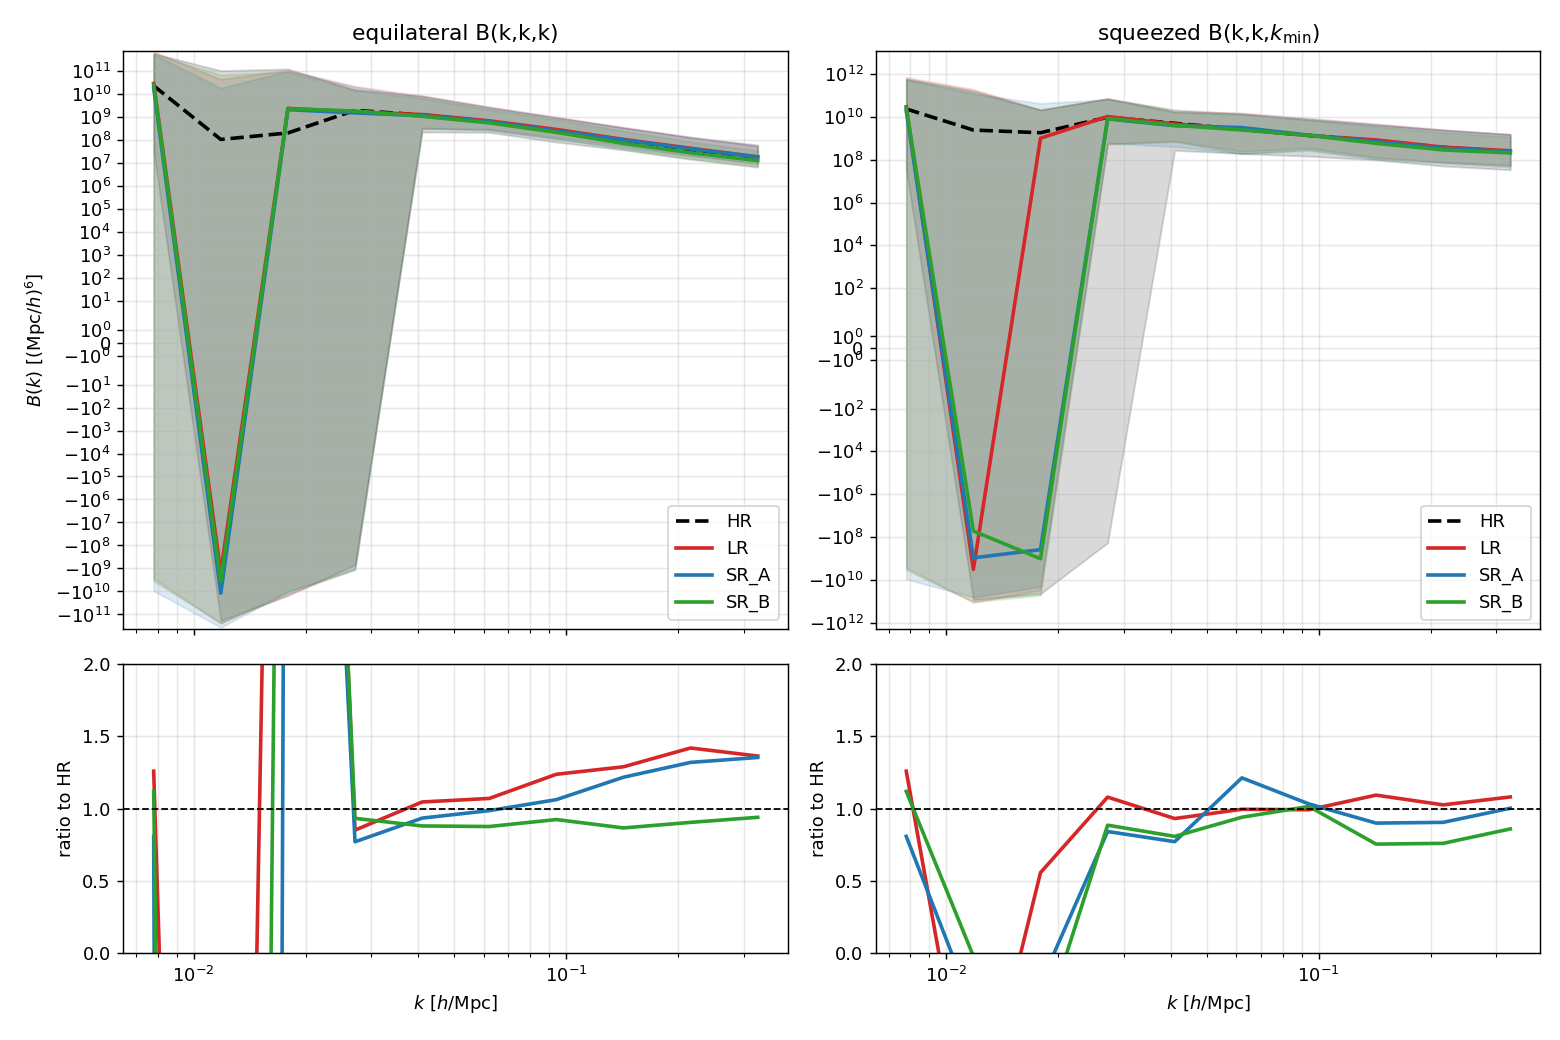
\includegraphics[width=0.95\linewidth]{figures_cmass/bispectrum_hr_lr_srA_srB.png}
\caption{Bispectrum of HR, LR, and SR (both arms), on $16$ test boxes. Top:
equilateral and squeezed bispectrum, HR in black. Bottom: ratio to HR. SR
removes most of the systematic excess that LR has at the plotted scales,
without ever training on this statistic.}
\label{fig:srs-bispec}
\end{figure}

On the equilateral configuration, LR sits about $6$ to $13$ percent above HR
across the middle range of scales. SR removes most of this gap without ever
seeing a bispectrum during training, and it does this for both arms. This is
evidence that the model is not simply fitting the training metric. It is
correcting real structure in the field that also shows up in a statistic it
never saw. (The figure uses the earlier models trained \emph{with} the power
spectrum loss; the no-Pk models of the following paragraphs preserve the
bispectrum at least as well, so removing that loss did not degrade this
held-out statistic either.)

\paragraph{Removing the power spectrum loss.} Following the meeting, we
retrained the model with the power spectrum term switched off
($\lambda_\text{pk}{=}0$ in Eq.~\ref{eq:srs-lossG}), so the loss is only the
adversarial and $L_1$ terms. We also changed which checkpoint counts as "best"
to the real-space $L_1$ error, since selecting on the power spectrum would
have been the same kind of leak we were trying to remove.

\begin{figure}[t]
\centering
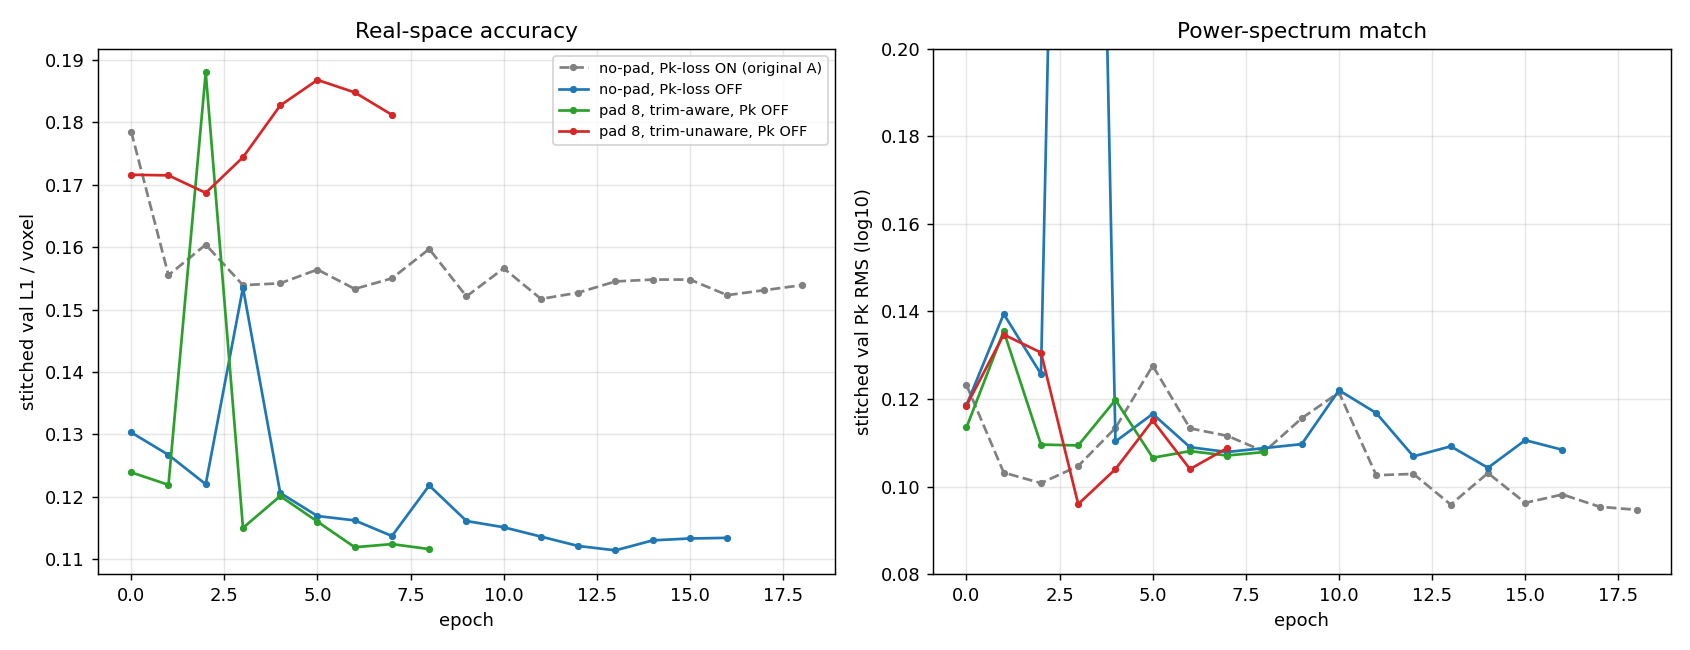
\includegraphics[width=0.98\linewidth]{figures_cmass/protocolv2_cmass.png}
\caption{Stitched validation curves under the new protocol (power spectrum
loss off). Left: real-space $L_1$ error. Right: power spectrum RMS error. Grey
dashed: the original Arm A with the power spectrum loss on, for comparison.
These runs are still training; curves stop at the most recent completed
epoch.}
\label{fig:srs-protocolv2}
\end{figure}

Two things stand out so far. First, without the power spectrum term, the
real-space $L_1$ error becomes clearly better than the original run at the
same point in training (left panel, blue and green curves sit below the grey
dashed curve). Second, the power spectrum error does get a little worse
without its loss term, but it does not collapse: it settles into roughly the
same range as before, just a bit noisier. So the power spectrum term was
buying us a small amount of power spectrum accuracy at a real cost in
real-space accuracy. It was not the only reason the power spectrum matched
well; the adversarial and reconstruction terms carry most of that on their
own.

\paragraph{Does padding help, once the power spectrum loss is out of the way?}
The report above found that padding (Arm B) did not beat no padding (Arm A) on
the power spectrum. The mentor pointed out two different ways this could
happen, and that they make different, testable predictions:
\begin{itemize}
  \item \textbf{Trim-aware.} The model is trained knowing that only the middle
  part of its output will be kept; the loss only looks at that middle part.
  This is what Arm B already did. If this is working correctly, padding should
  train at least as well as no padding, since it has strictly more context for
  the same target.
  \item \textbf{Trim-unaware.} The model is trained as if its whole padded
  output matters, including the edge region that gets thrown away later. If
  the model leans on that edge region during training, it should look fine
  during training but generalize worse once the edge is cut off at test time.
\end{itemize}
We trained both versions with the power spectrum loss off, so the comparison
is not confused by that term. Figure~\ref{fig:srs-protocolv2} shows all three
runs together (no padding, trim-aware padding, trim-unaware padding).

The trim-aware version (green) matches or beats no-padding (blue) on both
real-space error and power spectrum error at almost every epoch measured so
far. This supports the first prediction: once the model is told correctly what
part of its output is graded, more context helps rather than hurts. The
trim-unaware version (red) is clearly worse on real-space error than both
other runs, and does not close that gap as training continues. This supports
the second prediction: a model that is allowed to rely on the part of its
output that gets discarded at test time pays for that at test time. Put
together, the original result that padding did not help was most likely
caused by the power spectrum loss, not by padding itself.

We also reran the older, padding-with-power-spectrum-loss model for more
epochs to check whether it had simply not been trained long enough. Fifteen
additional epochs did not beat its early best score, so that run was not
undertrained; the training recipe, not the training time, was the limiting
factor.

\subsection{The Goal Metric: Corrected Cross-Fidelity Results}
\label{sec:srs-correction}

\paragraph{The bug.} After the analysis above, a routine physical sanity check
failed in a way that could not be real: the amplitude of the power spectrum had
essentially zero correlation with $\sigma_8$, and a fit of the power spectrum to
the five parameters explained only $0.2\%$ of the variance. The power spectrum
amplitude must scale with $\sigma_8$, so this pointed to a labeling error, not to
physics. Tracing it, we found that the processed count fields were written in
string-sorted simulation order ($0, 1, 10, 100, 1000, \dots$) while the cosmology
table is indexed numerically. Field number $k$ is therefore the halo field of
simulation string-sort$(k)$, not simulation $k$, so every field in the whole
pipeline was paired with the wrong cosmology. We proved this exactly: using the
original halo catalogs, the field halo count matches the catalog count under the
string-sort permutation for all $2000$ simulations, while the identity mapping
matches only the two fixed points. We corrected the cosmology table to field
order, backed up the old one, and patched the builder so it cannot regenerate the
wrong order.

\begin{figure}[h]
\centering
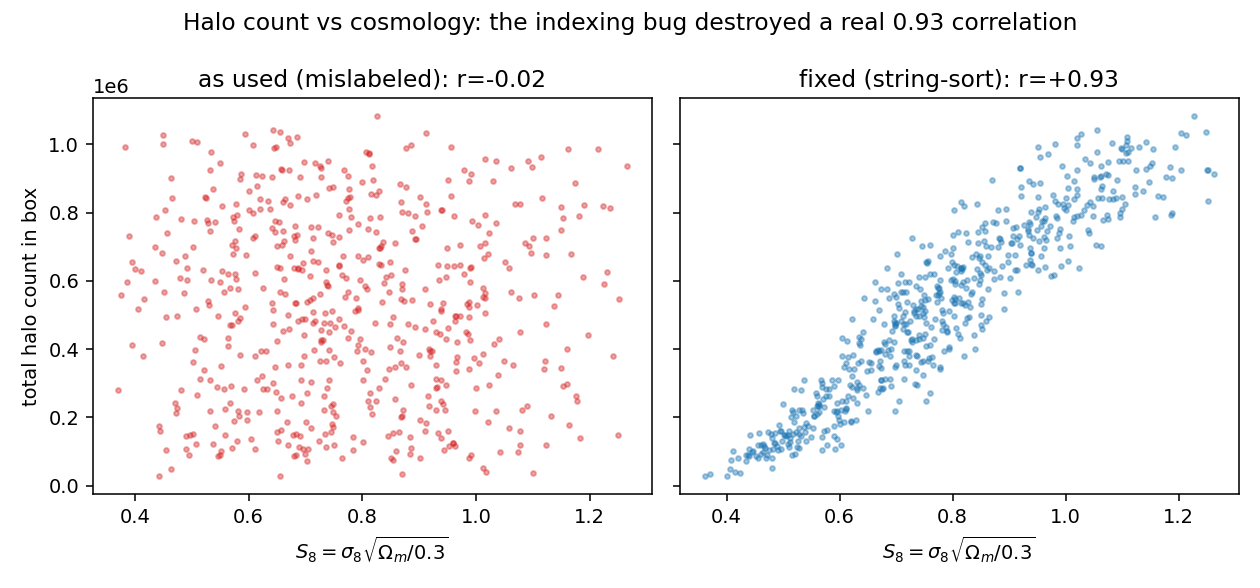
\includegraphics[width=0.85\linewidth]{figures_cmass/labelbug_count_vs_s8.png}
\caption{The indexing bug in one picture. Total halo count in a box against
$S_8 = \sigma_8\sqrt{\Omega_m/0.3}$. As the pipeline used the labels (left) the
correlation is zero; with the string-sort mapping corrected (right) the true
$0.93$ correlation reappears. Halo abundance must track $S_8$, so the left panel
was the signature of a labeling error, not of uninformative data.}
\label{fig:srs-labelbug}
\end{figure}

\paragraph{What this changes, and what it does not.} Every cosmology number we
computed before this point used the labels and is affected; the earlier
cross-fidelity tables have been removed and are replaced by the corrected results
below, and the earlier reading that the SR-versus-LR difference was an irreducible
coin flip was itself a product of the mislabeling. The results that do not use the
labels are unaffected and still stand: the power spectrum match of SR to HR, the
held-out bispectrum, the field-match statistics, the seam test, and the real space
error. The generator conditions on the cosmology as a style vector and was trained
with the scrambled labels, so its conditioning was uninformative during training;
we return to this at the end.

\paragraph{The data is informative after all.} With correct labels the picture
inverts. A halo count in this suite carries a strong cosmological signal: the
total halo count alone correlates with the combination $S_8 = \sigma_8
\sqrt{\Omega_m/0.3}$ at $0.93$ and with $\Omega_m$ at $0.85$. A Fisher forecast on
a single-box power spectrum now explains $98\%$ of the variance, where it
explained $0.2\%$ before, and it constrains $\Omega_m$ and $\sigma_8$ well, with
$\Omega_b$, $h$ and $n_s$ weak or unconstrained, which is the textbook pattern for
a low-redshift halo field. The field-level network tells the same story: after the
fix its predicted $\Omega_m$ correlates with the truth at $0.90$ on both training
and test boxes, where before the fix the correlation was zero and the output was a
constant. So the earlier conclusion that a single box carries almost no cosmology
was an artifact of the labeling, not a property of the data.

\begin{figure}[h]
\centering
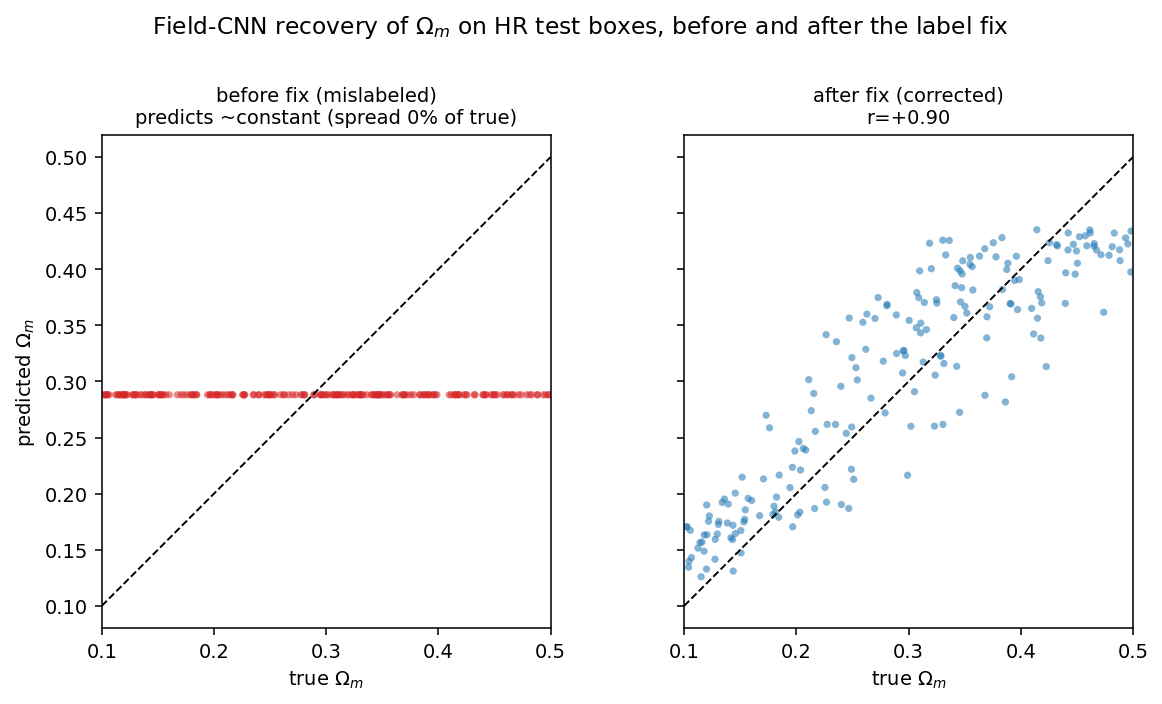
\includegraphics[width=0.82\linewidth]{figures_cmass/field_recovery_Om_cmass.png}
\caption{Field-level CNN recovery of $\Omega_m$ on HR test boxes, before and after
the label fix. Before (left) the prediction is flat and uncorrelated with the
truth (the network returns a near-constant); after (right) it tracks the diagonal
at a correlation of about $0.90$, on both training and test boxes. Same
architecture, same data, only the labels changed.}
\label{fig:srs-recovery}
\end{figure}

\begin{figure}[h]
\centering
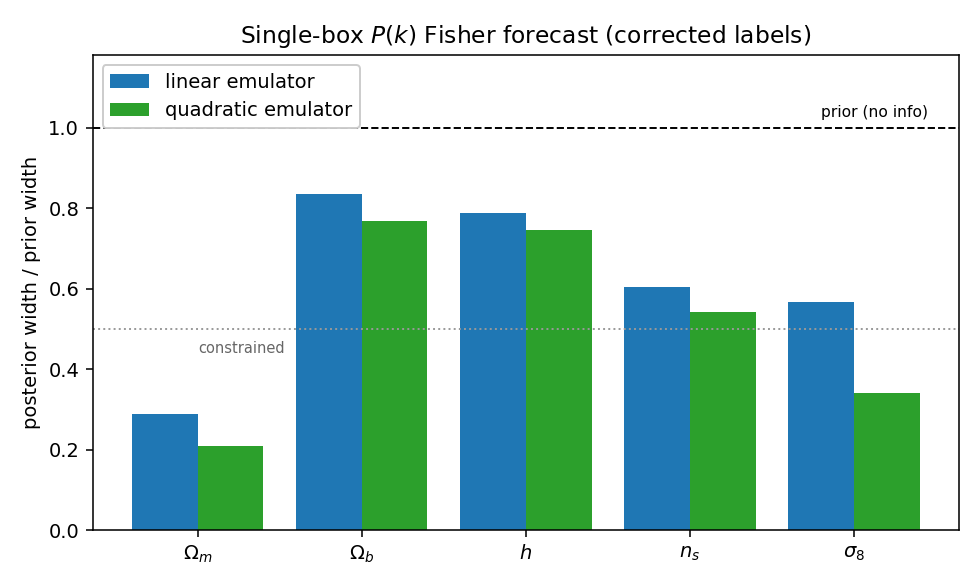
\includegraphics[width=0.72\linewidth]{figures_cmass/fisher_corrected_cmass.png}
\caption{Fisher forecast for a single-box power spectrum with corrected labels:
posterior width divided by prior width per parameter (lower means better
constrained, $1$ means no information). $\Omega_m$ is well constrained and
$\sigma_8$ is constrained, while $\Omega_b$, $h$ and $n_s$ are weak, the textbook
pattern for a low-redshift halo field. Two emulators (linear average slope and
quadratic at the prior centre) bracket the estimate.}
\label{fig:srs-fisher}
\end{figure}

\paragraph{Corrected cross-fidelity, and where SR helps.} We re-ran the goal
metric with correct labels at two levels, the power spectrum summary and the full
field. We train the posterior on one source, apply it to HR, and compare to a
posterior trained on HR, using an ensemble of independently retrained estimators
so the numbers are not single draws. Table~\ref{tab:srs-corrected} gives the
result.
\begin{table}[h]
\centering
\caption{Corrected cross-fidelity KL to HR (posterior trained on the named source,
evaluated on HR), lower is better, with the HR-to-HR floor for reference. Summary
uses the power spectrum; field uses a three-dimensional CNN posterior on the full
box.}
\label{tab:srs-corrected}
\begin{tabular}{lccc}
\toprule
level & LR (raw) & SR & HR floor \\
\midrule
summary $P(k)$ & $0.032$ & $0.088$ & $0.028$ \\
field (CNN)    & $0.49 \pm 0.81$ & $\mathbf{0.024}$ & $0.022$ \\
\bottomrule
\end{tabular}
\end{table}
\begin{figure}[h]
\centering
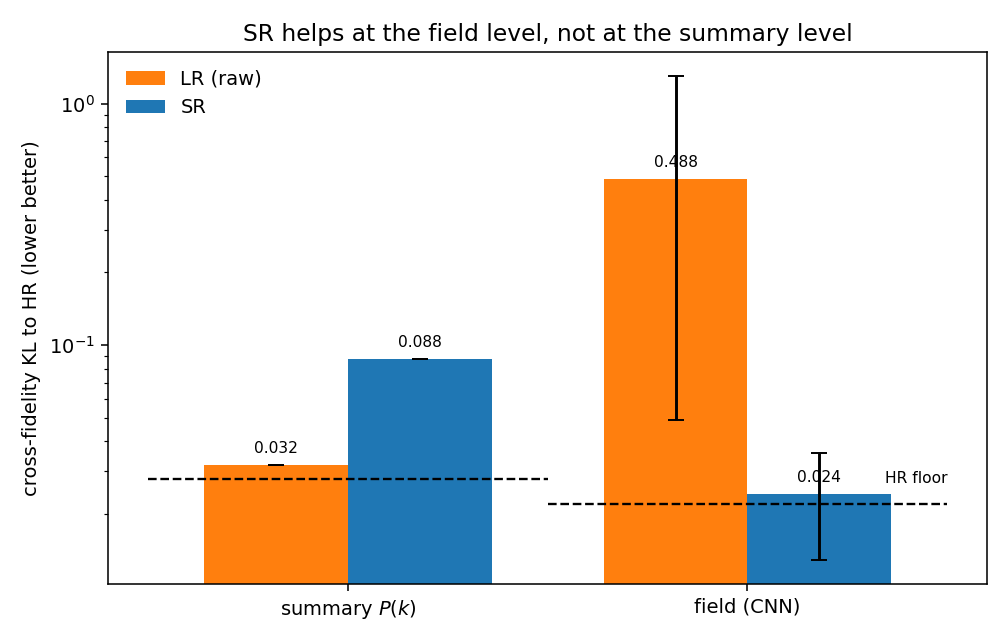
\includegraphics[width=0.7\linewidth]{figures_cmass/crossfid_corrected_cmass.png}
\caption{Corrected cross-fidelity KL to HR (log scale, lower is better) at the two
levels, with the HR-to-HR floor shown as the dashed line. At the summary level the
raw LR field is already at the floor and SR does not help. At the field level, an
LR-trained posterior does not transfer to HR (large and unstable), while an
SR-trained posterior sits at the floor. SR helps exactly where it corrects the
field.}
\label{fig:srs-crossfid-corrected}
\end{figure}
The two levels point in opposite directions, and both make sense. At the summary
level the raw LR power spectrum is already at the HR floor, so an LR-trained
posterior transfers to HR as well as an HR-trained one does, and there is no gap
for SR to close; SR even hurts a little, because the generator reshapes the
small-scale power in a way that does not match how HR responds to cosmology. At
the field level the raw LR box looks different enough from HR that an LR-trained
posterior does not transfer, and it does so unreliably, sometimes acceptably and
sometimes catastrophically, which is why its number carries such a large spread.
SR corrects the field to look like HR, so an SR-trained posterior transfers to HR
reliably, at the floor. This is exactly the deployment case the project is built
on, train the inference model on cheap SR-corrected boxes and apply it to
expensive HR, and at the field level SR makes it work where raw LR does not.

\paragraph{Padding on the goal metric.} We ran the two padding variants through
the corrected cross-fidelity at the summary level as well
(Table~\ref{tab:srs-padding}). Among the SR models the ordering from the earlier
report survives: no padding is best on the goal metric, trim-aware padding is
worse, and trim-unaware is worst, so for the cosmology objective the no-padding
model is the one to use. All three sit above the raw LR control at this level,
consistent with LR already being HR-like on the power spectrum. One number does
change under the fix: the mislabeled data made trim-unaware look catastrophic (a
factor of several hundred above the others), while with correct labels it is the
weakest variant by about a factor of two, not a blow-up. Its real-space error
(Figure~\ref{fig:srs-protocolv2}) remains the clearest and most direct sign that
it is the least reliable model.
\begin{table}[h]
\centering
\caption{Corrected cross-fidelity KL to HR at the summary (power spectrum) level
for the SR padding variants, with the LR control and the HR floor. Lower is
better. Field-level padding numbers are future work.}
\label{tab:srs-padding}
\begin{tabular}{lc}
\toprule
model & summary cross-fidelity KL \\
\midrule
SR, no padding & $\mathbf{0.087}$ \\
SR, trim-aware padding & $0.127$ \\
SR, trim-unaware padding & $0.172$ \\
\midrule
LR (control) & $0.031$ \\
HR floor & $0.028$ \\
\bottomrule
\end{tabular}
\end{table}

\paragraph{Bottom line.} With the labels fixed, the cosmology question has a
clear answer. The data constrains $\Omega_m$ and $\sigma_8$ from a single box. At
the power spectrum level the raw LR field is already HR-like, so SR is not needed
there and slightly hurts. At the field level, which is what SR actually corrects,
an SR-trained posterior transfers to HR at the floor while a raw LR one does not,
so SR provides a real and reliable cosmology benefit exactly where it operates.
Trim-unaware padding is still the weakest variant, worst on the goal metric and
on real-space error, though the label fix shrinks its apparent failure from
catastrophic to about a factor of two. Two honest caveats remain: the
field-level LR number has a wide spread and rests on a handful of retrained
networks, so the size of the gap should be firmed up with more seeds; and because
the generator was trained with the scrambled labels, its cosmology conditioning
was uninformative, so a retrain with correct conditioning may sharpen the SR
result further. Neither caveat changes the direction: with correct labels, SR
helps cosmology at the field level.

\paragraph{A data reliability note.} Partway through these runs, the shared
data storage this project reads from filled up completely, which caused a few
training jobs to fail with a file briefly appearing missing even though it was
not actually deleted. We added a retry step to the data loader and resumed
each affected run from its last saved checkpoint, so no real training progress
was lost. This is a shared infrastructure issue, not a problem with the data or
the method.

\subsection{Files}
\begin{itemize}\itemsep0pt
  \item Data and patching: \texttt{data/patch\_dataset\_cmass.py}
  (shared ops in \texttt{data/patch\_dataset\_real.py})
  \item Model: \texttt{map2map/models/styled\_srsgan.py}
  (\texttt{G\_correct}, \texttt{D\_const})
  \item Training: \texttt{train\_patch\_cmass.py};
  run script \texttt{scripts/train\_patch\_cmass.slurm}
  \item Inference and stitching: \texttt{infer\_stitch\_cmass.py}
  \item Seam eval: \texttt{analysis/eval\_seam\_cmass.py}
  \item Box / per-patch diagnostics: \texttt{analysis/diag\_cmass.py}
  \item SR-vs-HR match stats: \texttt{analysis/match\_stats\_cmass.py}
  \item SR-vs-HR power-spectrum figure: \texttt{analysis/plot\_sr\_vs\_hr.py}
  \item Bispectrum (held-out statistic): \texttt{analysis/bispectrum\_cmass.py}
  \item Training loss curves: \texttt{analysis/plot\_losses\_cmass.py}
  \item Cross-fidelity posterior evaluation: \texttt{evaluate.py} (SR-trained
  or LR-trained posterior evaluated on HR $P(k)$)
  \item Protocol-v2 (no-Pk-loss, padding-variant) training curves:
  \texttt{analysis/plot\_protocolv2\_cmass.py}
  \item Power spectrum on counts: \texttt{analysis/power\_spectrum.py}
  (estimator \texttt{counts}); differentiable training version
  \texttt{analysis/pk\_torch.py}
  \item Posterior and KL: \texttt{inference/nde.py}, \texttt{evaluate.py};
  end-to-end eval \texttt{scripts/eval\_cmass\_wrapper.slurm}
  \item Field-level posterior (three-dimensional CNN, moment-network loss):
  \texttt{models/field\_cnn.py}, \texttt{train\_field\_cnn.py};
  SR field generation \texttt{gen\_sr\_fields.py}; capacity and recovery
  diagnostics \texttt{overfit\_test.py}, \texttt{field\_diag.py}
  \item Outputs: \texttt{runs/patch\_cmass/}; figures: \texttt{figures\_cmass/}
\end{itemize}
